\documentclass[../hw10]{subfiles}

\begin{document}

\subsection*{Project}
Consider a projectile fired at an angle $\theta$, $\theta \in (0,\pi/2)$, from a point $(x_0, y_0)$ with initial velocity $v_0$. 
The horizontal component of $v_0$ is $v_0\cos{\theta}$, and the vertical component is $v_0\sin{\theta}$.
Let $x=x(t), \quad y=y(t)$ be parametric equations for the path of the projectile.

We neglect air resistance and the curvature of the earth. Under these circumstances there is no horizontal acceleration and, \[x''(t)=0.\]

The only vertical acceleration is due to gravity; therefore \[y''(t)=-g.\]

\subsubsection*{1}
Show that the path of the projectile (the trajectory) is given parametrically by the functions
\[x(t)=(v_0\cos{\theta})t+x_0, \quad y(t) = -\frac{1}{2}gt^2+(v_0\sin{\theta})t+y_0.\]

We begin with $x(t)$. We know that there is no horizontal acceleration. Given that acceleration is the second derivative of position, then $x''(t)=0$.

We integrate to reveal that $x'(t)$, the velocity, is some constant. This constant is the initial horizontal velocity $v_0\cos{\theta}$.

We then integrate, $\int x'(t)\,dt = \int v_0\cos{\theta}\,dt$, which is $x(t)=(v_0\cos{\theta})t$ with a constant. This constant is the initial position $x_0$.

So, $x(t)=(v_0\cos{\theta})t+x_0$, as desired.

We repeat this process for $y(t)$, noting that there is vertical acceleration due to gravity. So $y''(t)=-g$.

Then, $\int y''(t)\,dt = \int -g\, dt$ where the constant term of the resulting integral is the vertical velocity $v_0\sin{\theta}$.

So $y'(t)=-gt+v_0\sin{\theta}$. We then integrate once more, noting that the final constant of integration will be the initial vertical position $y_0$.

Thus, $y(t)=\int y'(t)\,dt = \int -gt+v_0\sin{\theta} \, dt = -\frac{gt^2}{2}+(v_0\sin{\theta})t+y_0$ as was given above.

\subsubsection*{2}
Show that in rectangular coordinates the equation of the trajectory can be written
\[y=-\frac{g}{2{v_0}^2}\sec^2{\theta}{(x-x_0)}^2+\tan{\theta}(x-x_0)+y_0.\]

First, we isolate $t$ in the equation for $x$,
\begin{align*}
    x&=(v_0\cos{\theta})t+x_0 \\
    \frac{x-x_0}{v_0\cos{\theta}}&=t. \\
\end{align*}

Then, we use this $t$ in $y(t)$,
\begin{align*}
    y(t) &= -\frac{1}{2}gt^2+(v_0\sin{\theta})t+y_0 \\
    y\left( \frac{x-x_0}{v_0\cos{\theta}} \right) &= -\frac{g}{2}{\left( \frac{x-x_0}{v_0\cos{\theta}} \right)}^2 + (v_0\sin{\theta})\left( \frac{x-x_0}{v_0\cos{\theta}} \right)+y_0 \\
    &= -\frac{g}{2{v_0}^2}\left( \frac{1}{\cos^2{\theta}}\right){(x-x_0)}^2 +v_0\left( \frac{\sin{\theta}}{\cos{\theta}}\right) (x-x_0) + y_0 \\
    &= -\frac{g}{2{v_0}^2}\sec^2{\theta}{(x-x_0)}^2+\tan{\theta}(x-x_0)+y_0.
\end{align*}

\subsubsection*{3}
Measure distances in feet, time in seconds, and set $g=32$ft/sec$^2$. 
Take $(x_0,y_0)$ as the origin and the $x$-axis as ground level.
Consider a projectile fired at an angle $\theta$ with initial velocity $v_0$.

\begin{enumerate}[label=\alph*.]
    \item Give parametric equations for the trajectory; give an equation in $x$ and $y$ for the trajectory.
    \item Find the range of the projectile, which in this case is the $x$-coordinate of teh point of impact.
    \item How many seconds after firing does the impact take place?
    \item Choose $\theta$ so at to maximize the range.
    \item Choose $\theta$ so that the projectile lands at $x=b$.
\end{enumerate}

For (a), from (1) along with $(x_0,y_0)=(0,0)$, we get
\[x(t)=(v_0\cos{\theta})t, \quad y(t)=\frac{-gt^2}{2}+(v_0\sin{\theta})t.\]

For (b), we wish to find $t$ such that $y=0$. With $y(0)=0$ given, we proceed with $t\neq0$. So,
\begin{align*}
    y(t)=0&=\frac{-gt^2}{2}+(v_0\sin{\theta})t \\
    0 &= t(v_0\sin{\theta}-\frac{gt^2}{2}), \quad t\neq0 \\
    0 &= v_0\sin{\theta} - \frac{gt^2}{2} \\
    t &= \frac{2v_0\sin{\theta}}{g}. \\
\end{align*}

If the projectile is fired at $t_i=0$, then $t_f=\frac{2v_0\sin{\theta}}{g}$ is the time at which the projectile impacts the ground.

The range of the projectile $x$, since $x(0)=0$, is then $x(t)$ at the impact time $t_f$. We compute,
\begin{align*}
    x(t) &= (v_0\cos{\theta})t \\
    x(t_f) &= (v_0\cos{\theta})\left( \frac{2v_0\sin{\theta}}{g} \right) \\
    &= \frac{2{v_0}^2}{g}\cos{\theta}\sin{\theta}. \\
\end{align*}

For (c), we already computed that the impact time occurs at $t=\frac{2v_0}{g}\sin{\theta}$ seconds in (b).

For (d), we note that the range of the projectile at the impact time $t_f$ is $\frac{2{v_0}^2}{g}\cos{\theta}\sin{\theta}$. 

We will optimize this value for theta. We define the range as a function of theta, \[l(\theta)=\frac{2{v_0}^2}{g}\cos{\theta}\sin{\theta}.\]

We compute $l'(\theta)$ and equate this value to zero to find the critical points of $l$.
\begin{align*}
    l&=\frac{2{v_0}^2}{g}\cos{\theta}\sin{\theta} \\
    l'&=\frac{2{v_0}^2}{g}\left( \cos^2{\theta} - \sin^2{\theta}\right) \\
    0&=\frac{2{v_0}^2}{g}\left( \cos^2{\theta} - \sin^2{\theta}\right) \\
    0&=\cos^2{\theta}-\sin^2{\theta} \\
    \sin^2{\theta}&=\cos^2{\theta} \\
    \tan{\theta}&=1 \\
    \theta&=\tan^{-1}{1} \\
    \theta&=\frac{\pi}{4}. \\
\end{align*}

Thus, $\theta=\frac{\pi}{4}$ optimizes the distance $x$ that the projectile travels.

For (e), we desire $\theta$ such that $l(\theta)=b$.
So, we equate,
\begin{align*}
    b&=\frac{2{v_0}^2}{g}\cos{\theta}\sin{\theta} \\
    \frac{bg}{2{v_0}^2}&=\cos{\theta}\sin{\theta}; \\
\end{align*}
We use the double angle identity, \[\frac{1}{2}\sin{2x}=\cos{x}\sin{x}.\]
Then,
\begin{align*}
    \frac{bg}{2{v_0}^2}&=\frac{\sin{2\theta}}{2} \\
    \frac{bg}{{v_0}^2}&=\sin{2\theta} \\
    \sin^{-1}{\frac{bg}{{v_0}^2}} &= 2\theta \\
    \frac{1}{2}\sin^{-1}{\frac{bg}{{v_0}^2}} &= \theta. \\
\end{align*}

So, the angle required to impact the projectile at $x=b$ is $\theta=\frac{1}{2}\sin^{-1}{\frac{bg}{{v_0}^2}}$.

\subsubsection*{4}

\begin{enumerate}[label=\alph*.]
    \item Graph the path of the projectile fired at an angle of $\frac{\pi}{6}$ with initial velocity $v_0=1500$ft/sec. Determine the range of the projectile and the heigh reached.
    \item Keeping $v_0=1500$ft/sec, experiment with several values of $\theta$. Confirm that $\theta=\pi/4$ maximizes the range. What angle maximizes the height reached? 
\end{enumerate}

For (a), we will first determine the maximum height and range of the projectile. From 3(b), we know that the range of the projectile is given by $\frac{2{v_0}^2}{g}\cos{\theta}\sin{\theta}$. So, with the given launch angle and velocity, we see that the range $l$ is,
\begin{align*}
    l&=\frac{2\cdot{1500}^2}{32}\cos{\frac{\pi}{6}}\sin{\frac{\pi}{6}} \\
    &=\frac{2250000}{166}\left( \frac{\sqrt{3}}{2} \right)\left( \frac{1}{2} \right) \\
    &=\frac{140625\sqrt{3}}{4} \\
    &\approx 60892
\end{align*}

So the projectile travels about 60892 feet.

For the height of the projectile, we note that the projectile will be at its maximum height halfway through its trajectory path. We can also compute this $t_{\max}$ by finding the critical points of $y(t)$.

We use $y'(t)$ from (1), equating the expression to zero,
\begin{align*}
    y'(t)&=-gt+v_0\sin{\theta} \\
    0&=-gt_{\max}+v_0\sin{\theta} \\
    t_{\max}&=\frac{v_0\sin{\theta}}{g}. \\
\end{align*}

We note that $t_{\max}$ is exactly half of $t_f$.

We continue to find $y\left( t_{\max} \right)$ to determine the maximum height of the projectile.
\begin{align*}
    y(t)&=\frac{-gt^2}{2}+(v_0\sin{\theta})t \\
    y(t_{\max})&=\frac{-g}{2}{\left(\frac{v_0\sin{\theta}}{g}\right)}^2+v_0\sin{\theta}\left(\frac{v_0\sin{\theta}}{g}\right) \\
    &=-\frac{1}{2}\frac{{(v_0\sin{\theta})}^2}{g}+\frac{{(v_0\sin{\theta})}^2}{g} \\
    &= \frac{{(v_0\sin{\theta})}^2}{2g}.
\end{align*}

We then use the given conditions to finish solving for the height $h$,
\begin{align*}
  h&=\frac{{(1500\sin{\frac{\pi}{6}})}^2}{2\cdot32} \\
  &= \frac{{(750)}^2}{64} \\
  &= \frac{562500}{64} \\
  &= \frac{140625}{16} \\
  &\approx 8489.
\end{align*}

Therefore, the maximum height of the projectile is about 8489 feet.

We then graph the motion of the projectile.
\begin{figure*}[ht]
\centering
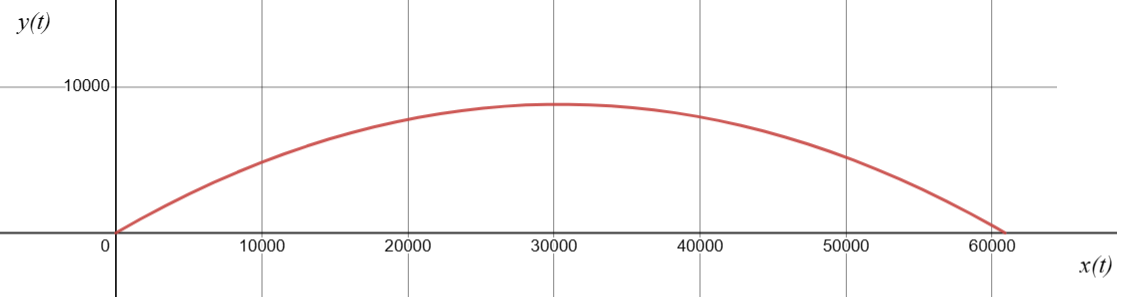
\includegraphics[width=0.8\linewidth]{../content/figure1.png}
\caption{Trajectory of projectile with launch angle $\pi/6$ and initial velocity 1500 ft/sec.}
\end{figure*}

For (b), we have already analytically confirmed that $\theta=\frac{\pi}{4}$ maximizes the range of the projectile for any initial velocity. 

We might expect that a different launch angle would maximize the height reached by the projectile, however. We predict that shooting the projectile directly upwards, at an angle of $\theta=\frac{\pi}{2}$, will result in the maximum height attained.

We then optimize the maximum height $h$ from (a), noting that the launch angle is bounded between 0 and $\pi/2$.
\begin{align*}
    h&=\frac{{(v_0\sin{\theta})}^2}{2g} \\ 
    h'&=\frac{{v_0}^2}{2g}(2\sin{\theta}\cos{\theta}) \\
    0&=\frac{{v_0}^2}{2g}(2\sin{\theta}\cos{\theta}) \\
    0&=\cos{\theta}\sin{\theta} \\
    0,\frac{\pi}{2}&=\theta.
\end{align*}

We get a critical point for $h$ when $\theta$ is either $0$ or $\frac{\pi}{2}$. 

We first examine $\theta=0$, noting that this will result in a maximum height of zero given that $\sin{0}=0$ for the sine term in $h$. 

Thus, it is our angle of $\frac{\pi}{2}$ that produces a maximum height.

Then, the maximum height for a given initial velocity $v_0$ is given by,
\begin{align*}
    h_{\max}&=\frac{{(v_0\sin{\frac{\pi}{2}})}^2}{2g} \\
    &=\frac{{v_0}^2}{2g}.
\end{align*}

\end{document}